\subsubsection{The Rayleigh-Taylor instability}
\label{sec:benchmark-rayleigh-taylor}

\textit{This section was contributed by Cedric Thieulot.}

This benchmark is carried out in \cite{Deu08,Ger10,thie11} and is
based on the analytical solution by Ramberg\cite{ramb68},
which  consists of a gravitationally unstable two-layer system.
Free slip are imposed on the sides while no-slip boundary conditions are imposed on the
top and the bottom of the box.
Fluid 1 $(\rho_1,\eta_1)$ of thickness $h_1$ overlays
fluid 2 $(\rho_2,\eta_2)$ of thickness $h_2$ (with $h_1+h_2=L_y$).
An initial sinusoidal disturbance of the interface between these
layers is introduced and is characterised by an amplitude $\Delta$ and a
wavelength $\lambda=L_x/2$ as shown in Figure~\ref{fig:RTi_setup}.

\begin{figure}
  \centering
  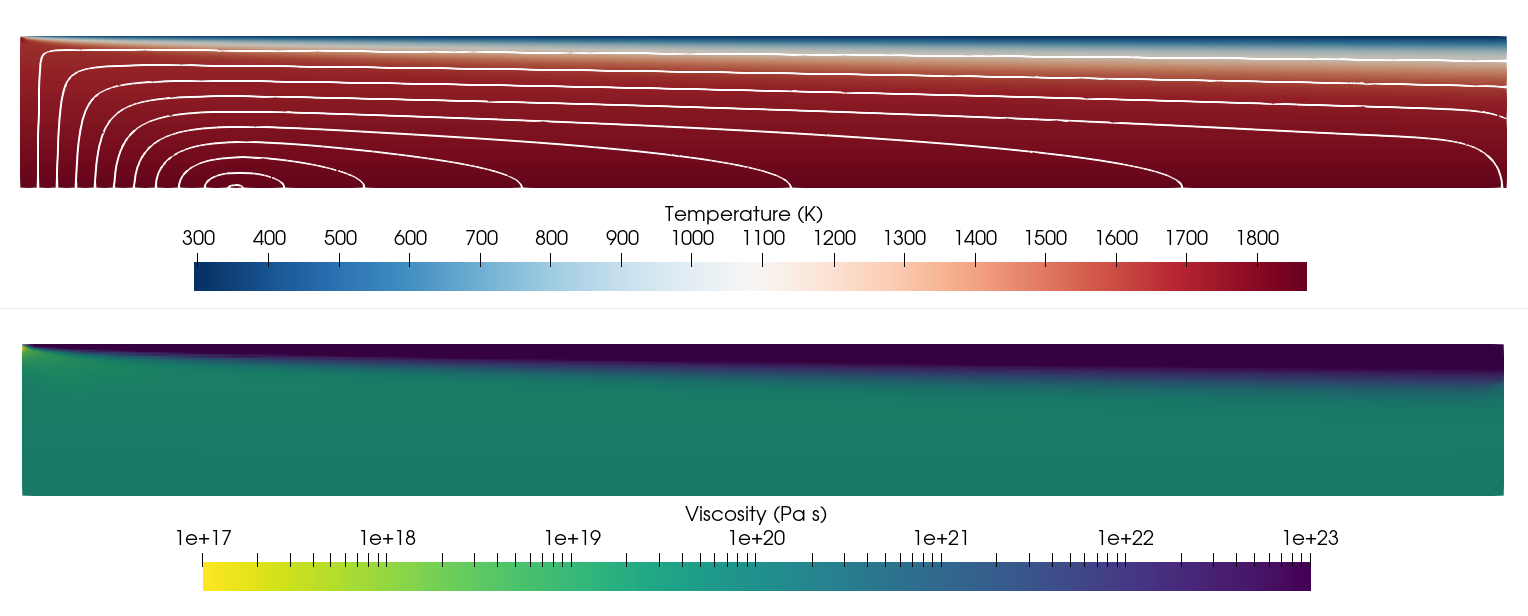
\includegraphics[width=0.4\textwidth]{cookbooks/benchmarks/rayleigh_taylor_instability/doc/setup}
  \caption{\it Setup of the Rayleigh-Taylor instability benchmark (taken from \cite{thie11})}
  \label{fig:RTi_setup}
\end{figure}

Under this condition, the velocity of the diapiric growth
$v_y$ is given by the relation
\begin{equation}
\frac{v_y}{\Delta} = - K \frac{\rho_1-\rho_2}{2 \eta_2} h_2 g
\qquad
\qquad
\text{with}
\qquad
\qquad
K=\frac{-d_{12}}{c_{11}j_{22}-d_{12}i_{21}}
\end{equation}
where $K$ is the dimensionless growth factor and
\begin{eqnarray}
c_{11} &=& \frac{\eta_1 2 \phi_1^2}{\eta_2(\cosh 2\phi_1 - 1 - 2\phi_1^2)} - \frac{2\phi_2^2}{\cosh 2\phi_2 - 1 - 2 \phi_2^2}\\
d_{12} &=& \frac{\eta_1(\sinh 2\phi_1 -2\phi_1)}{\eta_2(\cosh 2\phi_1 -1 -2\phi_1^2)} + \frac{\sinh 2\phi_2 - 2\phi_2}{\cosh 2\phi_2 -1 -2\phi_2^2} \\
i_{21} &=& \frac{\eta_1\phi_2 (\sinh 2 \phi_1 + 2 \phi_1)}{\eta_2(\cosh 2\phi_1 -1 -2\phi_1^2)}
+ \frac{\phi_2 (\sinh 2\phi_2 + 2\phi_2)}{\cosh 2\phi_2 -1 -2\phi_2^2} \\
j_{22} &=& \frac{\eta_1 2 \phi_1^2 \phi_2}{\eta_2(\cosh 2\phi_1 -1-2\phi_1^2)} - \frac{2\phi_2^3}{ \cosh 2\phi_2 -1 -2\phi_2^2}\\
\phi_1&=&\frac{2\pi h_1}{\lambda} \\
\phi_2&=&\frac{2\pi h_2}{\lambda}
\end{eqnarray}
We set $L_x=L_y=\SI{512}{km}$, $h_1=h_2=\SI{256}{km}$, $|\boldsymbol{g}|=\SI{10}{m/s^2}$, $\Delta=\SI{3}{km}$,
$\rho_1=\SI{3300}{kg/m^3}$, $\rho_2=\SI{3000}{kg/m^3}$, $\eta_1=\SI{1e21}{Pa.s}$. $\eta_2$ is varied between $10^{20}$ and $10^{23}$
and 3 values of $\lambda$ (64, 128, and 256km) are used.
Adaptive mesh refinement based on density is used to capture the interface between the two
fluids, as shown in Figure~\ref{fig:RTi_grids}. This translates as follows in the input file:
\begin{verbatim}
subsection Mesh refinement
  set Initial global refinement = 4
  set Initial adaptive refinement = 6
  set Strategy = density
  set Refinement fraction = 0.6
end
\end{verbatim}

\begin{figure}
  \centering
  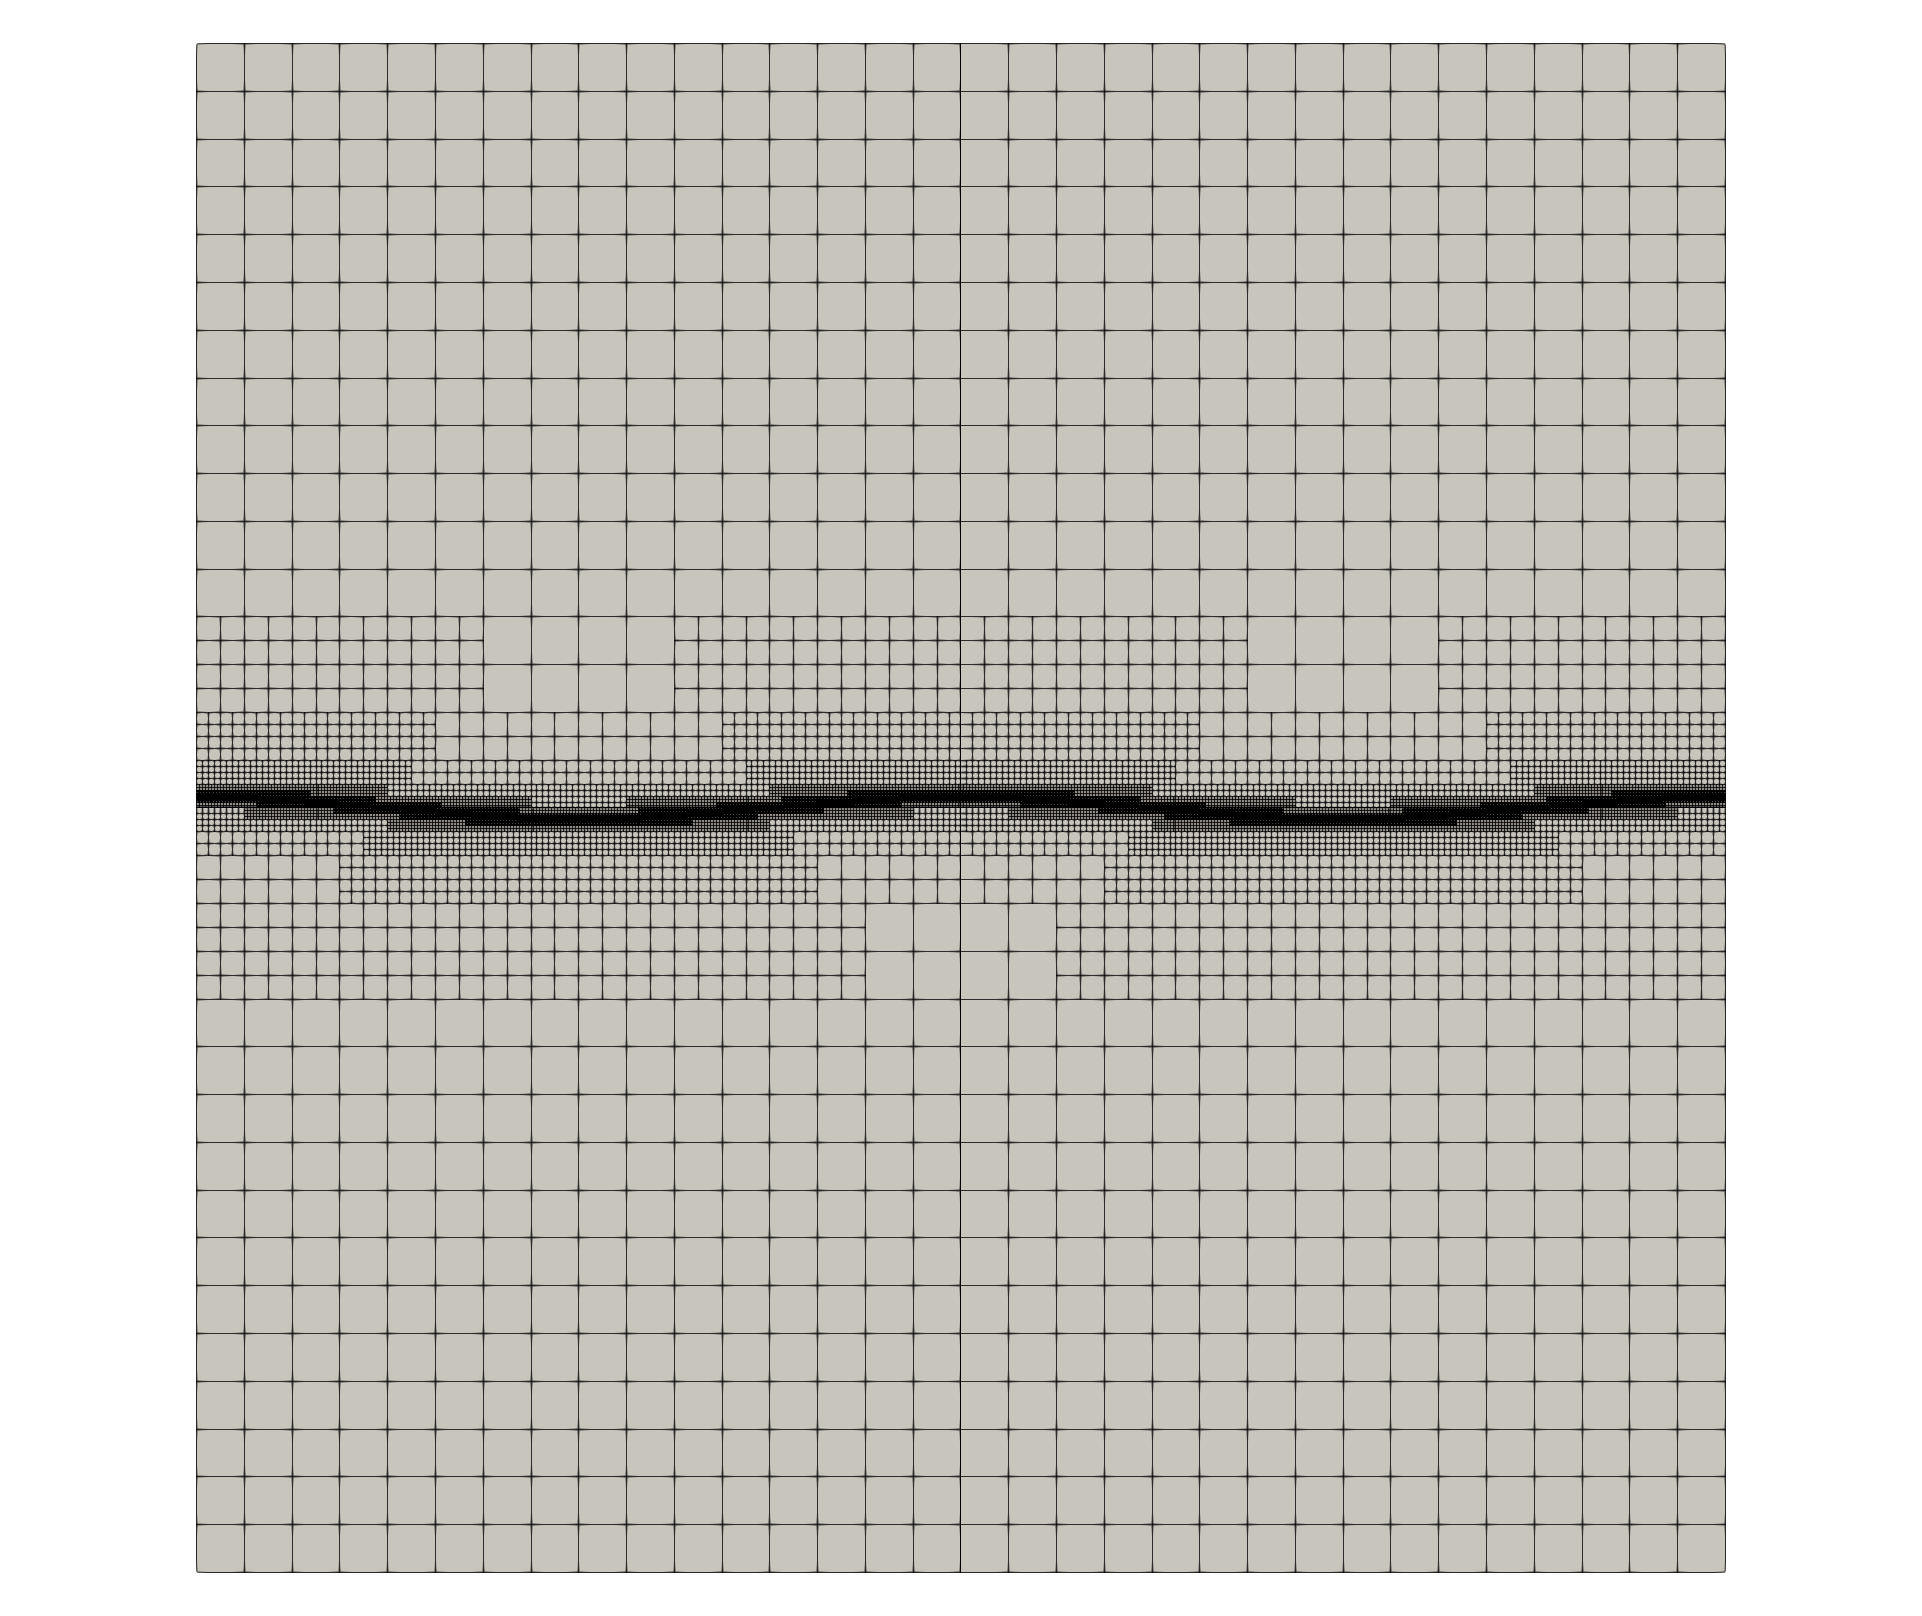
\includegraphics[width=0.44\textwidth]{cookbooks/benchmarks/rayleigh_taylor_instability/doc/grid}
  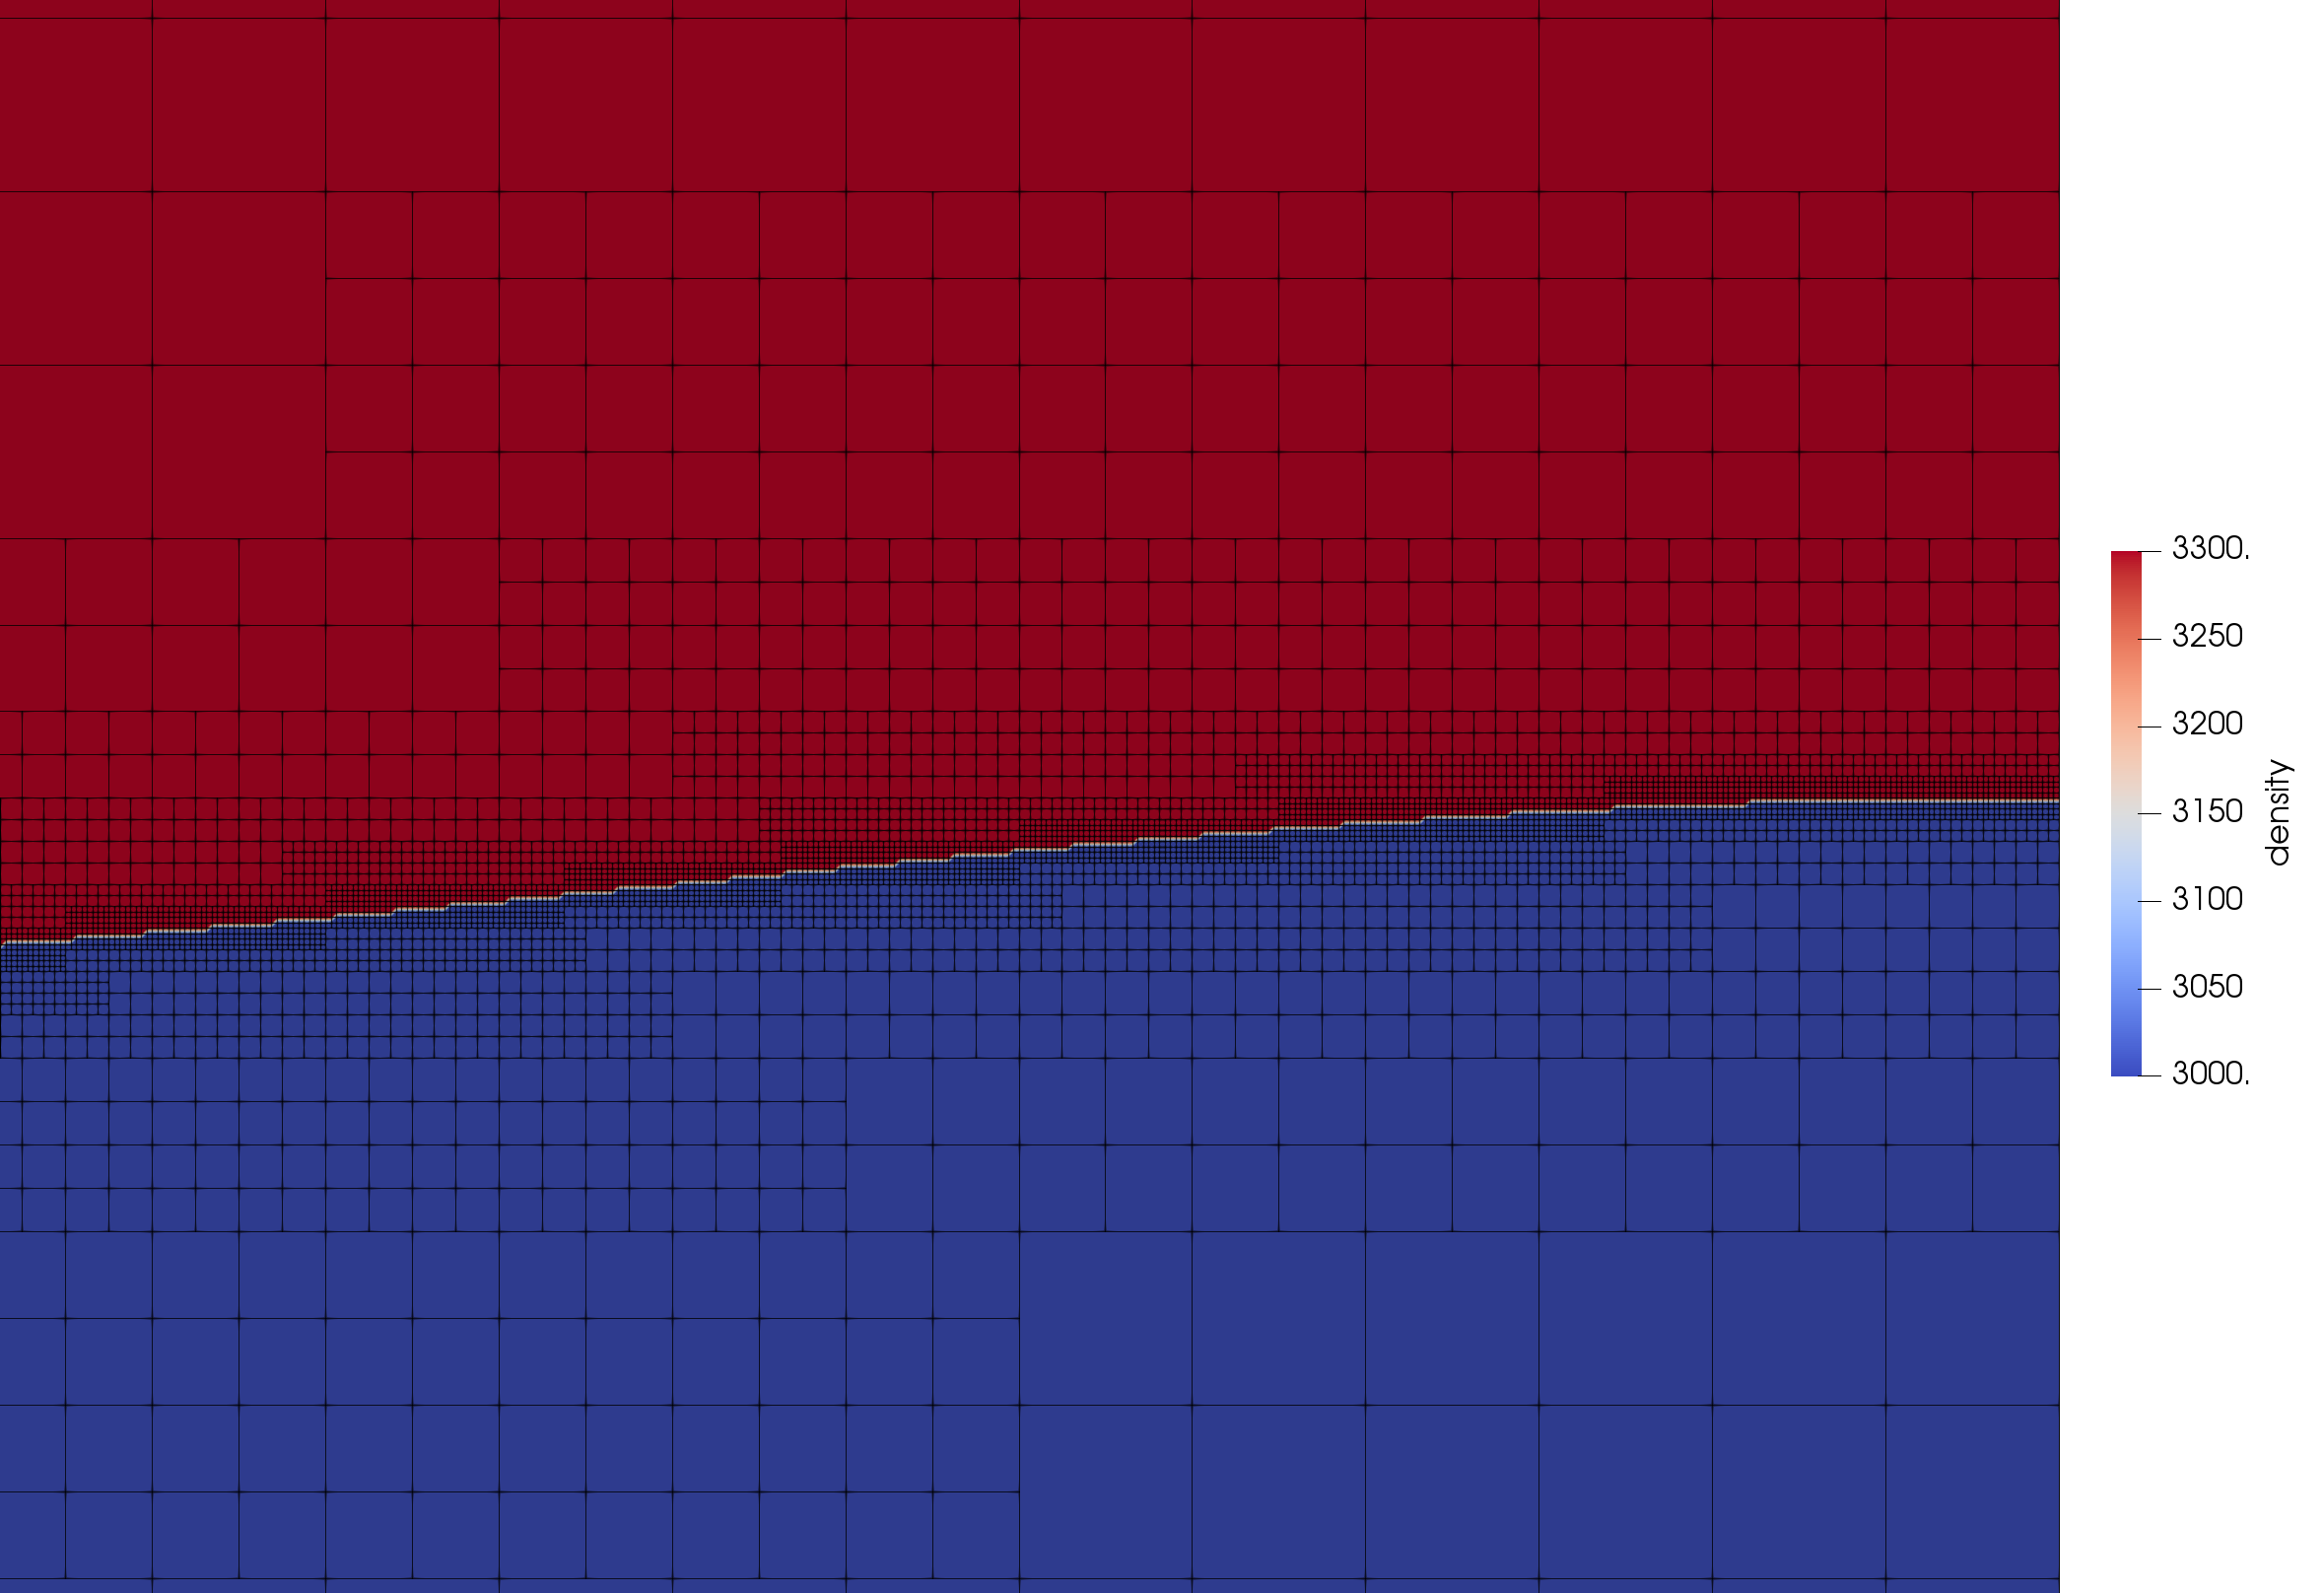
\includegraphics[width=0.52\textwidth]{cookbooks/benchmarks/rayleigh_taylor_instability/doc/grid2}
  \caption{\it Left: grid with initial global refinement 4 and adaptive refinement 6; Right: density field with detail of the mesh.}
  \label{fig:RTi_grids}
\end{figure}

The maximum vertical velocity is plotted against $\phi_1$ in Figure~\ref{fig:RTi_vels} and is found to match analytical results.

\begin{figure}
  \centering
  \includesvg[width=0.75\textwidth]{cookbooks/benchmarks/rayleigh_taylor_instability/doc/plot.svg}
  \caption{\it Maximum velocity for three values of the $\phi_1$ parameter.}
  \label{fig:RTi_vels}
\end{figure}
